%
% file : learn_git.tex
% date : jeudi 19 décembre 2019, 13:19:09 (UTC+0100)
% author : sedelpeuch
% description :
\documentclass[a4paper,10pt]{article}
\usepackage[utf8]{inputenc}
\usepackage[T1]{fontenc}
\usepackage[french]{babel}
\usepackage{graphicx}
\usepackage{float}
\usepackage{amsmath}
\usepackage{amssymb}
\usepackage{mathrsfs}
\usepackage{color}
\usepackage{fancyhdr}
\usepackage{pdfpages}
\usepackage{layout}
\usepackage{multicol}
\usepackage{setspace}
\usepackage{csvsimple}
\usepackage[table]{xcolor}
\usepackage[colorlinks=true]{hyperref}
\usepackage{tikz, tkz-tab}
\usepackage[top=2cm,bottom=2cm,left=2cm,right=2cm]{geometry}
\usepackage{amsthm}
\usepackage{listings}
\usepackage{verbatim}
\usepackage{transparent}
\usepackage{eso-pic,graphicx}

\AddToShipoutPicture*{
    \unitlength=0cm
    \put(0,0){\includegraphics{filigramme3.png}}

}
\AddToShipoutPicture{%
  \unitlength=1cm
    \put(1.6,8){\transparent{0.3}\includegraphics[width=18cm,
        height=13cm]{filigrame.png}}
  }

\setlength{\parindent}{0.785cm}
\setlength{\parskip}{1ex plus 0.5ex minus 0.2ex}
\newcommand{\hsp}{\hspace{20pt}}
\newcommand{\HRule}{\rule{\linewidth}{0.1mm}}
\newcommand{\therule}{\rule{5cm}{0.05mm}}


\usepackage{xcolor}
\begin{document}
\begin{spacing}{1.5}
\graphicspath{{image/}}
  \begin{titlepage}
\begin{sffamily}
\begin{center}
  \vspace*{\stretch{1}}
\textbf{\textsc{\LARGE Eirbot \\ Association de robotique de
    l'ENSEIRB-MATMECA}}\\[1cm]
\HRule \\[0.2cm]
       {\Huge \bfseries \fontsize{30}{30}\selectfont Présentation des projets 2020 \\
       \HRule \\[0.5cm]

\vspace*{\stretch{1}}
       \includegraphics[scale=0.4]{LogoEirbot.png}
       \vfill}
  \end{center}
  \end{sffamily}
\end{titlepage}
\setcounter{tocdepth}{2}
\newpage
\pagestyle{fancy}
\lhead{}
\chead{\textbf{Présentation des projets 2020}}
\rhead{\thepage}
\lfoot{}
\cfoot{}
%% \section*{Qui sommes nous ?}
%% Association de robotique de l'ENSEIRB-MATMECA crée en 2003, Eirbot est avant
%% tout un groupe de passionné d'électronique, d'informatique et de mécanique.
%% Chaque année, Eirbot acceuille un certain nombre d'élève ingénieur de première,
%% deuxième et troisième année. Cette année l'association contient une trentaine de membre
%% actifs. \\
%% Forte d'une équipe motivée, diversifiée, stimulée et soudée nous nous réunissons
%% autour d'un projet commun : la coupe de france de robotique. \\
%% Eirbot participe depuis sa création en tant que club (en 1997) à la coupe de
%% France de robotique
%% Les objectifs de l'association sont les suivants
%% \begin{itemize}
%% \item Participation à la coupe de France de robotique à la Roche sur Yon tous
%% les ans
%% \item Formations des éléves à la création d'un robot de A à Z (design/routage
%% de cartes électroniques, design de pièces 3D et impression 3D, initiation aux
%% systèmes embarqués)
%% \item Participation aux robots Maker's Day et autres évéenements organisés
%% dans l'école
%% \item transmission du savoir entre les anciens et les nouveaux adhérents
%% Nous disposons d'un local avec plusieurs outils mécanique et électroniques
%% (scies à chantourner, fer à souder, imprimante 3D, etc) situé dans l'enceinte
%% de l'école.
%% \end{itemize}
%% L'association est en partie finans l'objectif de continuer nos activités au
%% mieux, nous sommes à la recherche de partenariats. Ce derniers peuvent être de
%% toutes formes.
%% \newpage
\section*{Notre projet : coupe de France de robotique édition 2020}
Cette année, Eirbot prend le large ! Nos robots doivent partir voguer à travers
le monde. Nous allons devoir maîtriser la navigation pour arriver à bon port.
C'est après une tempête qu'il faudra reconstruire le chenal, réactiver le phare
et redresser les manches à air pour espérer gagner. Nos robots évolueront sur la
table suivante
\begin{figure}[H]
  \center
  \includegraphics[scale=0.2]{table.png}
  \caption{Schéma de la table de jeu}
\end{figure}
En plus de l'environnement de jeu nous devons suivre des règles précises
disponibles sur ce \href{https://www.coupederobotique.fr/wp-content/uploads/Eurobot2020_Rules_Cup_OFFICIAL_FR.pdf}{lien}.
Cette année Eirbot mise sur la qualité plutôt que la quantité : le robot
autonome aura pour objectif de faire avec précision les actions qu'il
entreprendra. L'objectif sera alors de construire et réactiver le phare, de redresser les
manches à air et de retourner à bon port après avoir décodé la boussole.

\subsection*{Plans du robot : des bases solides pour un bon départ}
Les plans de notre robot ont été réalisés. Ils ont pu devenir concrets grâce à la
découpe laser du FabLab de l'ENSEIRB MATMECA et à notre imprimante 3D. En
addition des profilés ont été utilisés pour monter la structure et créer des
étages faciles à monter et démonter.
\begin{figure}[H]
  \center
  \includegraphics[scale=0.3]{1A2020.png}
  \caption{Etat actuel de notre robot}
\end{figure}
Concernant notre phare, il doit se déployer et réaliser un balayage lumineux (il
doit faire moins de 30 cm avant l'activation et plus de 70 cm après).
Nous avons choisi l'impression d'un bras robotique pour notre phare, le système
d'éclairage du phare sera similaire à celui d'un vrai phare. Voici
l'avancement actuel
\begin{multicols}{2}
\begin{figure}[H]
  \center
  \includegraphics[scale=0.3, height=8cm]{phare_r.png}
  \caption{Etat actuel de notre phare replié}
\end{figure}
\columnbreak
\begin{figure}[H]
  \center
  \includegraphics[scale=0.3, height=8cm]{phare_d.png}
  \caption{Etat actuel de notre phare déplié}
\end{figure}
\end{multicols}
\subsection*{Fonctionnement général du robot : un contrôle précis pour une
  stratégie avancée}
Comme dit précédemment Eirbot mise sur la qualité de nos actions plutôt que la
quantité. Le travail informatique a donc été divisé en deux parties. D'une
part l'asservissement qui est implémenté sur une Nucléo-F429ZI. D'autre part, la
stratégie qui est implémentée sur une Raspberry pi 3b+. En addition un protocole
de communication entre les deux cartes a été créé.

Nous pouvons commencer par décrire succinctement l'asservissement que nous avons
élaboré. L'étape d'asservissement est cruciale. L'idée est que l'on puisse demander
au robot d'avancer d'une certaine distance et qu'il donne les bonnes consignes
aux moteurs pour réaliser cette distance avec le moins d'erreur possible.
Sans cela les stratégies qui seront mises en place par le suite ne pourront pas
aboutir.

Avec un asservissement précis nous pouvons réaliser une stratégie plus complexe.
Ainsi la stratégie dépend de deux facteurs principaux, la capacité à naviguer
sur la table et la capacité à détecter les adversaires et à réagir lorsque l'un
d'eux se présente. Pour la navigation un algorithme A* a été implémenté. C'est
un algorithme de recherche de chemin connu dérivé de l'algorithme de Dijikstra.
Le principe de ce dernier est résumé sur cette
\href{https://fr.wikipedia.org/wiki/Algorithme_A*#/media/Fichier:Astar_progress_animation.gif}{animation}\footnote{\url{https://fr.wikipedia.org/wiki/Algorithme_A*}}.
%% Nous avons modélisé la table comme une grille chaque case faisant $1 cm \times 1
%% cm$. Ainsi nous avons pu renseigner la position de tous les obstacles fixes. A
%% partir de cela nous pouvons expliquer le fonctionnement de l'algorithme. l'A*
%% commence à un noeud choisi. Il applique à ce dernier un coût initial, il estime
%% ensuite la distance entre ce noeud et le but à atteindre. Le noeud est alors
%% ajouté à une liste d'attente prioritaire, appelée \textit{open list}. \\ \indent
%% Premièrement l'algorithme récupère le premier noeud de l'\textit{open list}. Si
%% elle est vide, il n'y a aucun chemin du noeud initial à celui d'arrivée,
%% l'algorithme est en erreur. Si le noeud est celui d'arrivée, l'algorithme va
%% reconstruire le chemin complet et renvoyer le résultat. Ensuite, si le noeud
%% n'est pas le noeud d'arrivée alors de nouveaux noeuds sont créés pour tous les
%% noeuds contigus admissibles . L'A* calcule ensuite son coût et le stocke avec le
%% noeud. Ce coût est calculé à partir de la somme du coût de son ancêtre et du
%% coût de l'opération pour atteindre ce nouveau noeud. En parallèle l'algorithme
%% conserve la liste des noeuds qui ont été vérifiés, c'est la \textit{closed
%%   list}. Si un noeud nouvellement produit est déjà dans cette liste avec un coût
%% égal ou inférieur, on ne fait rien. Après, l'évaluation de la distance du
%% nouveau noeud au noeud d'arrivée est ajoutée au coût pour former l'heuristique
%% du noeud. Ce noeud est alors ajouté à la liste d'attente prioritaire, à moins
%% qu'un noeud identique dans cette liste ne possède déjà une heuristique
%% inférieure ou égale. Une fois ces étapes effectuées pour chaque nouveau noeud
%% contigu, le noeud original pris de la file d'attente prioritaire est ajouté à la
%% liste des noeuds vérifiés. Le prochain noeud est alors retiré de la file
%% d'attente prioritaire et le processus recommence.

Les détails techniques de l'implémentation sont disponibles sur le
\href{https://github.com/eirbot/eirbot2020-1A/blob/master/code/rasp/src/navigation.cpp}{Github}\footnote{\url{https://github.com/eirbot/eirbot2020-1A/blob/master/code/rasp/src/navigation.cpp}}
de l'association.
A ce stade, l'algorithme est opérationnel et il nous permet d'un point $x,y$
donné rejoindre n'importe quel point $x',y'$ en évitant les obstacles fixes.
Nous allons maintenant présenter notre stratégie concernant les obstacles
mobiles c'est-à-dire les adversaires.

Un système infrarouge (GP2) est utilisé pour la détection, ces derniers sont
placés juste au dessus des gobelets disposés sur la table (les gobelets sont
considérés comme des obstacles fixes, nous ne voulons pas les détecter avec le
système infrarouge). Lorsque un robot adverse est détecté, nous récupèrons l'information sur la distance fournie par le
système infrarouge, puis nous évitons l'obstacle. A ce stade nous avons un
système de détection nous permettant d'éviter les robots adverses en les
contournant.

Nous avons présenté nos principales stratégies mais nous n'avons pas décrit tous
nos codes. Les autres codes sont disponibles sur
notre dépot
\href{https://github.com/eirbot/eirbot2020-1A}{Github}\footnote{\url{https://github.com/eirbot/eirbot2020-1A}}.

En choisissant de séparer les codes sur deux cartes différentes, nous avons une
difficulté supplémentaire qui apparait. Il faut réaliser un protocole de
communication permettant d'envoyer des ordres de la carte maître (Raspberry Pi)
vers la carte esclave (Nucléo). Cette dernière répond aux commandes par une
action (déplacement, activation des actionneurs, ...) ou par des informations
sur l'état du robot (position, capteurs de distance, ...). Nous avons choisi
d'établir la communication via un port série et nous avons créé un protocole
spécifique aux besoins de notre projet. Le protocole implémente un système de
confirmation des commandes. Prenons un exemple simple, lorsque nous lançons la
Navigation sur la Raspberry pi, l'A* va calculer les positions à rejoindre. Au
fur et à mesure que l'algorithme trouve les positions il envoie une requête de
déplacement via le port série, attend la réponse du protocole et s'il n'y a pas
de soucis envoie la prochaine instruction.

\subsection*{Electronique du robot : une architecture sur mesure}
Pour que un robot fonctionne correctement, il a besoin d'être alimenté. La
conception d'une carte d'alimentation est une étape fondamentale lors de la mise
en oeuvre d'un projet de robotique. Cette dernière assure l'alimentation du
circuit à une tension souhaitée. La stabilité du signal doit être également
maintenue malgré les pertubations liées au circuit. Pour le robot, nous avons
opté pour une carte comportant 3 rails d'alimentation.

\begin{figure}[H]
  \center
  \includegraphics[scale=0.3]{carte.png}
  \caption{Etat actuel de notre carte d'alimentation}
\end{figure}

Deux de ces rails fournissent une alimentation de 5V,le premier alimente les
microcontroleurs, le suivant les actionneurs. Le dernier est consacré aux moteurs,
alimenté en 12V.

Mis à part les composants, l'intégralité de la carte a été conçue par nos soins
. La conception est effectuée grâce au logiciel Kickad et la réalisation est
possible dans l'enceinte de l'ENSEIRB-MATMECA. Le perçage des trous et la soudure des éléments se réalise
avec le matériel de l'association.

En plus de l'alimentation du robot ce dernier utilise deux moteurs pour se
déplacer. Il faut designer une carte de puissance afin de pouvoir les contrôler.
Cette carte fait la liaison entre l'alimentation, la carte Nucleo et les moteurs
eux-mêmes. Les cartes de puissances sont actuellement en cours de fabrication.

\newpage
\section*{Nos projets antérieurs}
Notre association possède une certaine ancienté et en plus de participer à la
coupe de France nous réalisons plusieurs projets voici quelques photos des
projets et des robots des années précédentes
\begin{multicols}{2}
  \begin{figure}[H]
    \center
    \includegraphics[scale=0.3]{1A2018.png}
  \end{figure}
  \columnbreak
  \begin{figure}[H]
    \center
    \includegraphics[scale=0.3]{1A2018_2.png}
  \end{figure}
\end{multicols}

\begin{multicols}{2}
  \begin{figure}[H]
    \center
    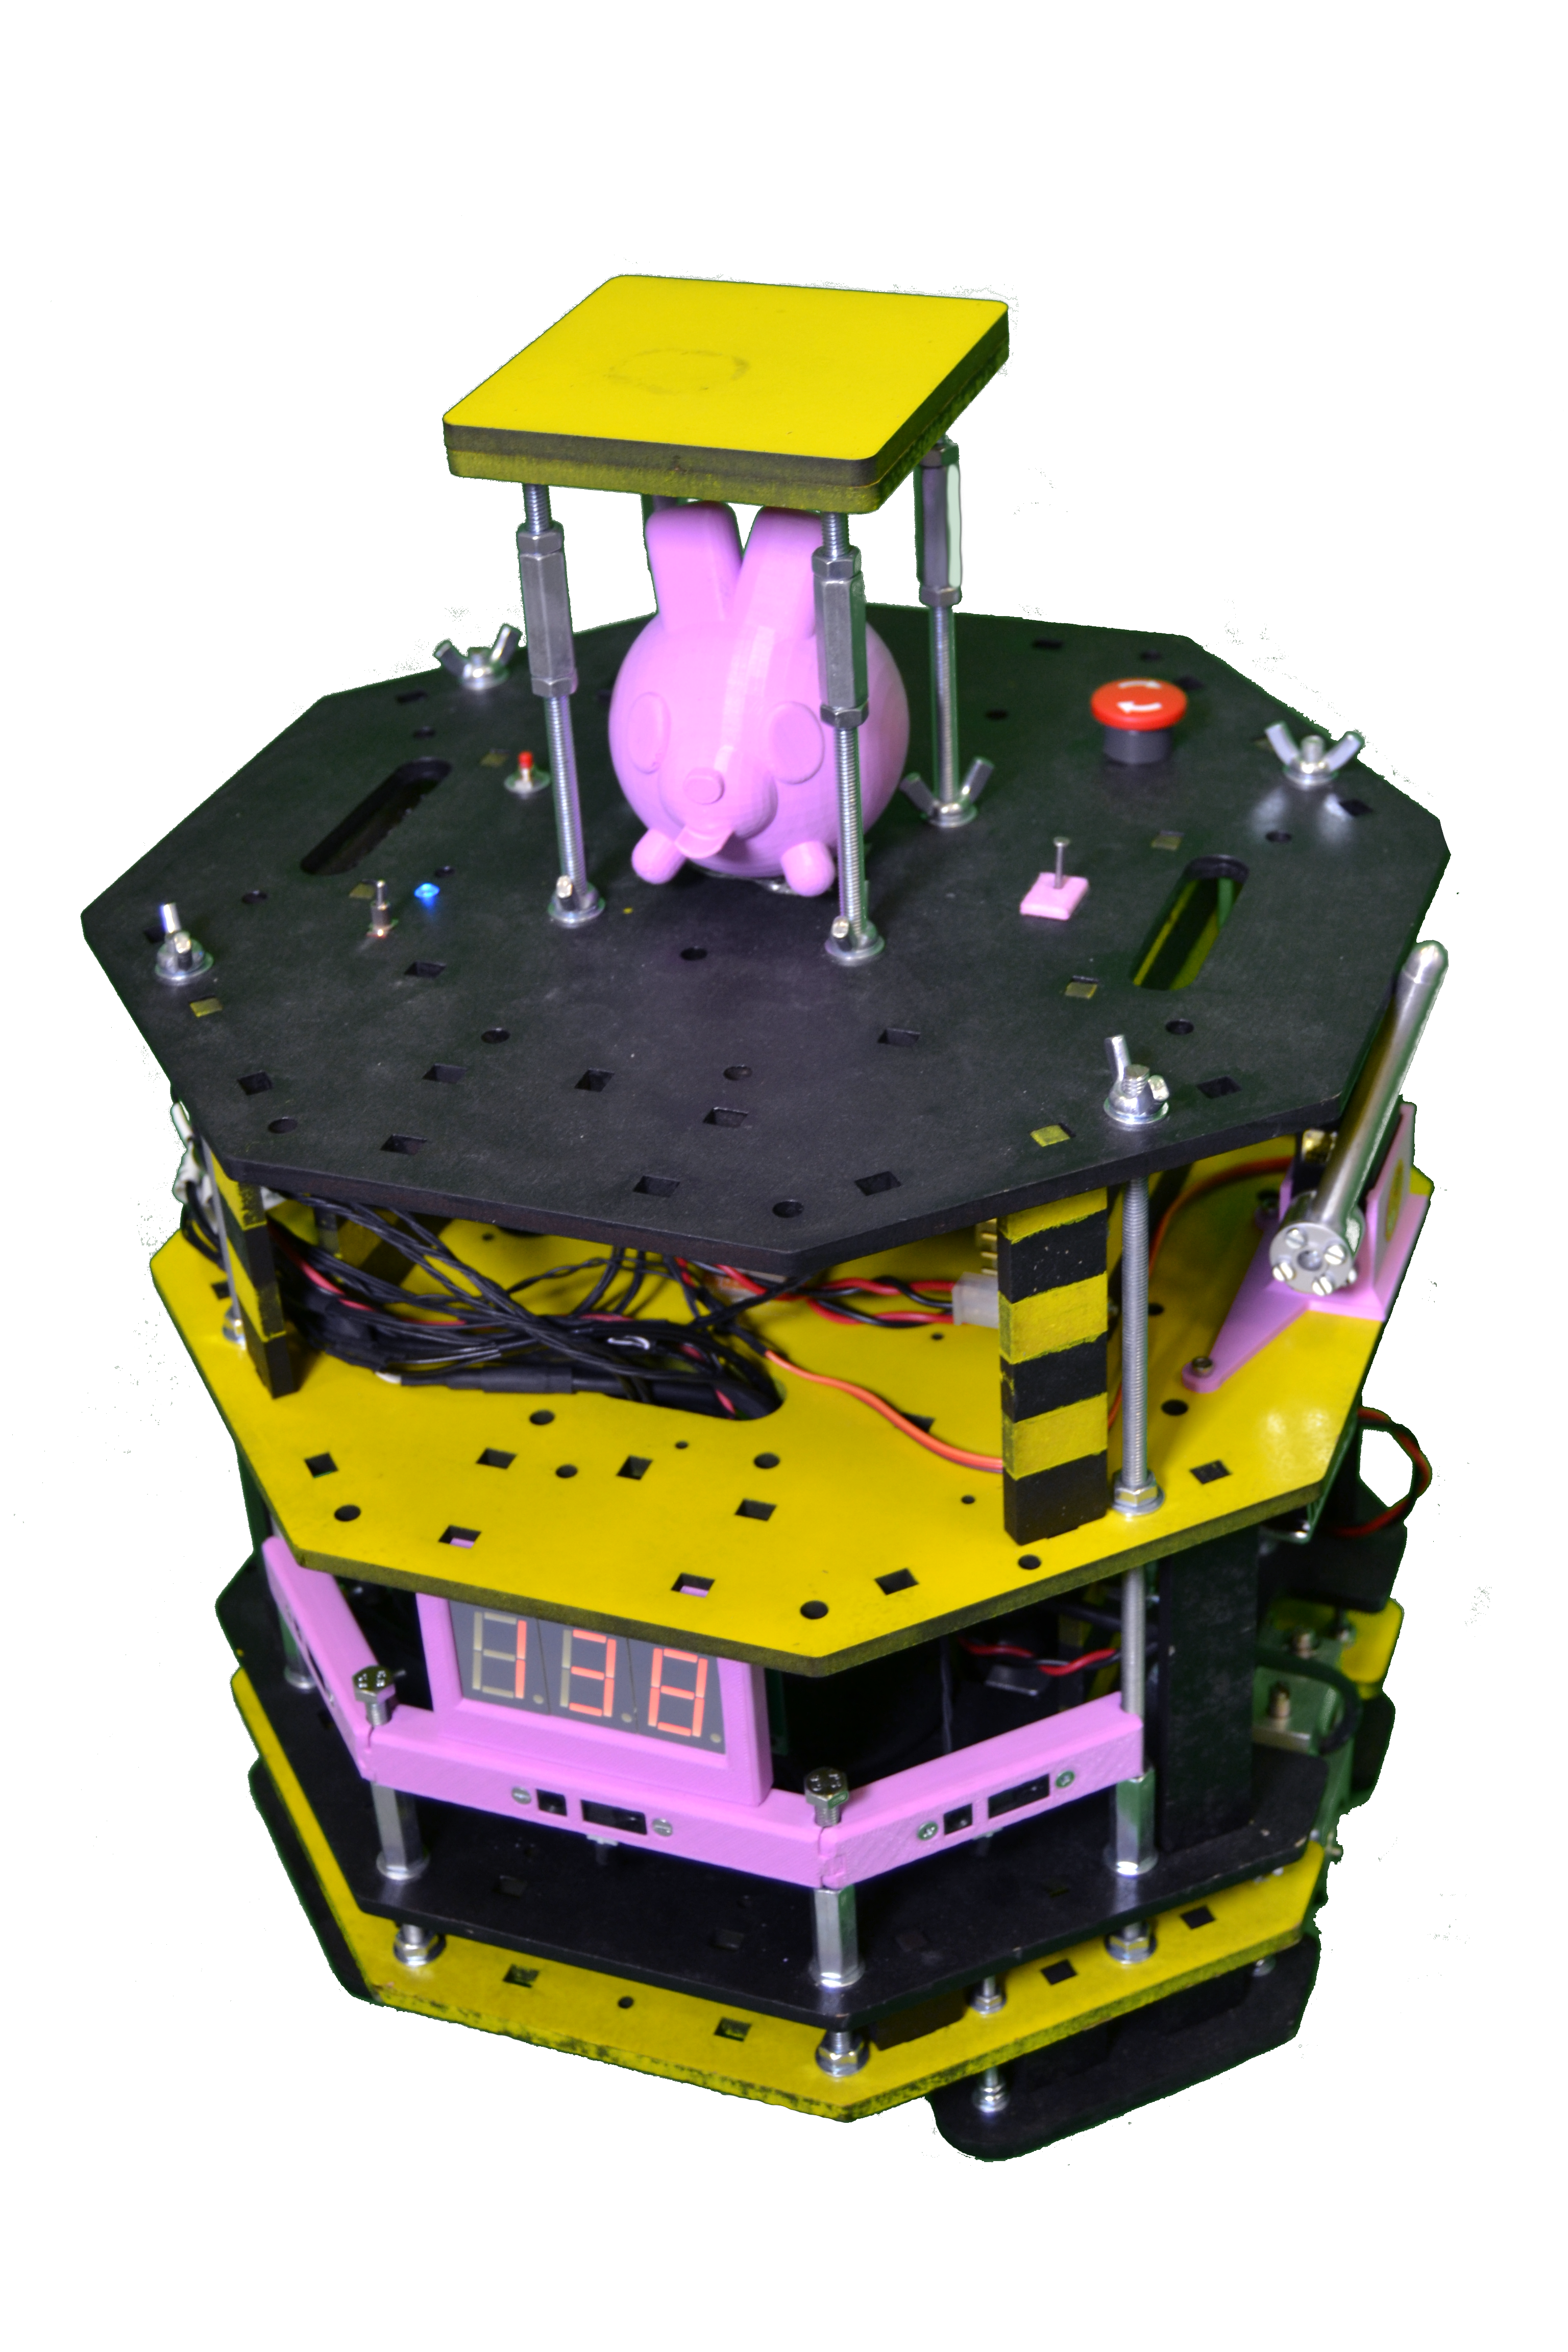
\includegraphics[scale=0.3]{2A2018.png}
  \end{figure}
  \columnbreak
  \begin{figure}[H]
    \center
    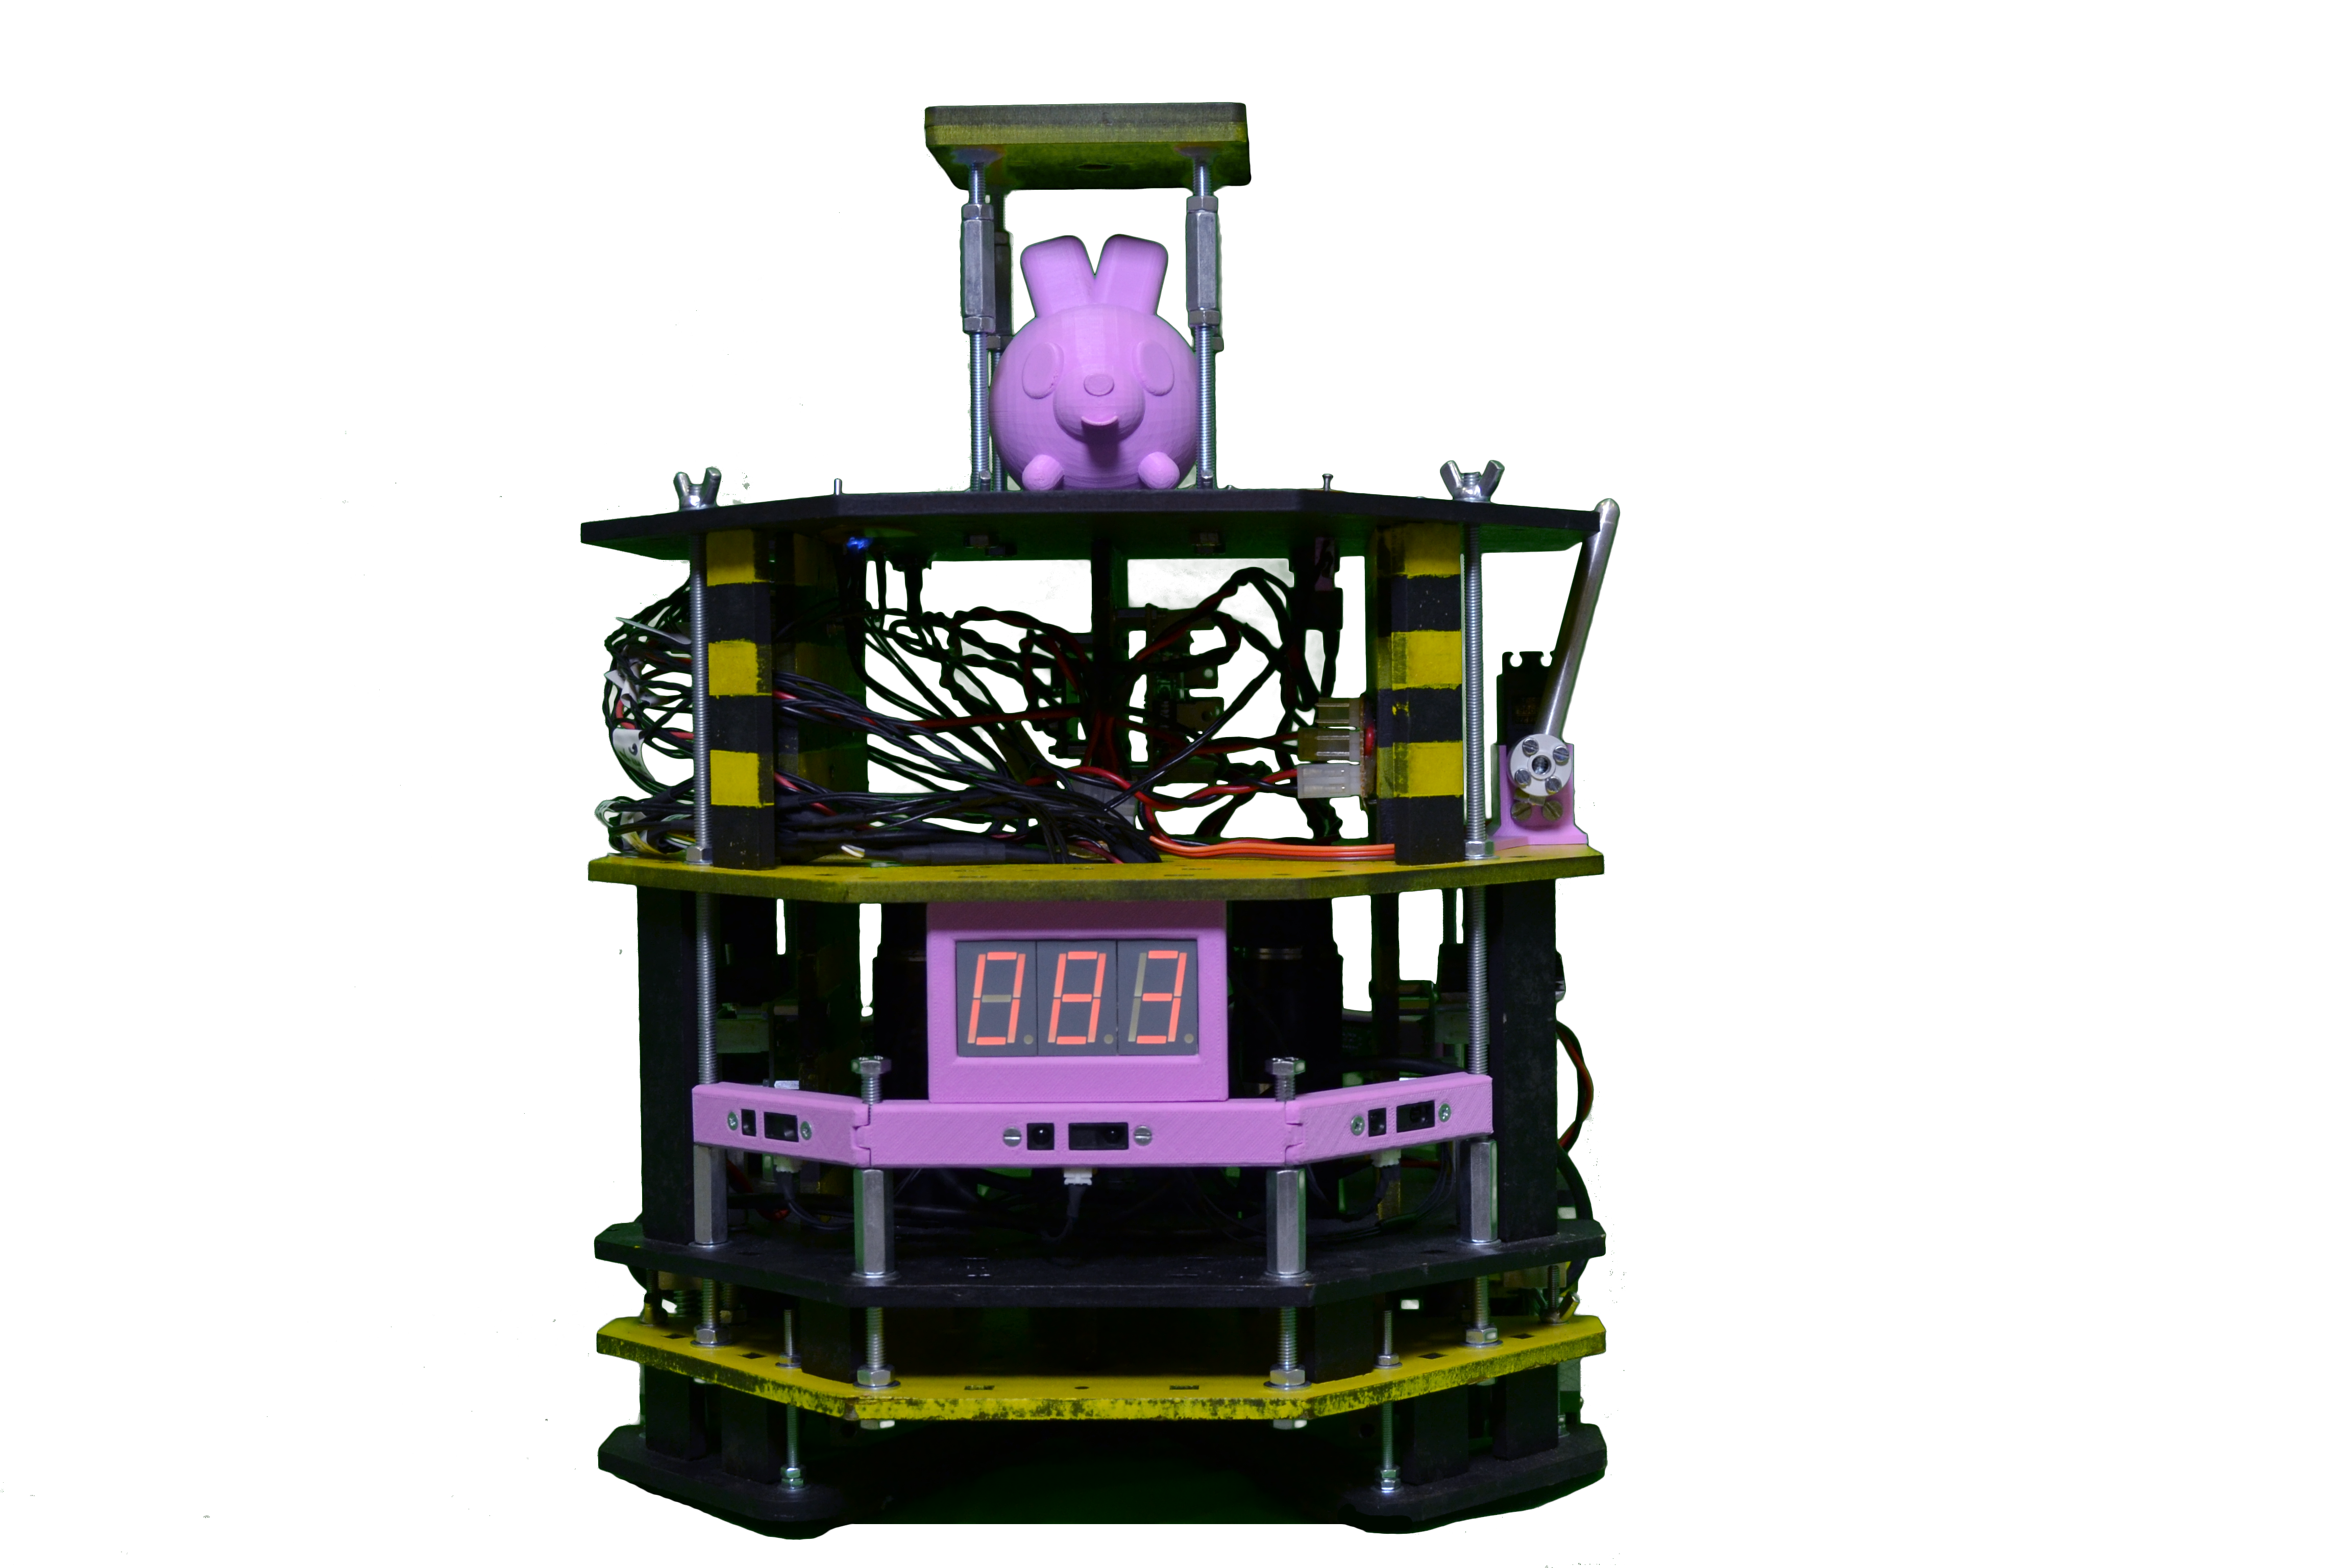
\includegraphics[scale=0.3]{2A2018(2).png}
  \end{figure}
\end{multicols}

  \begin{figure}[H]
    \center
    \includegraphics[scale=0.45]{brenda.png}
  \end{figure}

\begin{multicols}{2}
  \begin{figure}[H]
    \center
    \includegraphics[scale=0.2]{rubix_cube.jpg}
  \end{figure}
  \columnbreak
  \begin{figure}[H]
    \center
    \includegraphics[scale=0.2]{tourne.jpg}
  \end{figure}
\end{multicols}

\newpage
\end{spacing}
\end{document}
%%Brouillon du mail
%%
%%Bonjour,
%%Suite à notre discussion à l'afterwork Cdiscount organisé par AEI, je vous
%%envoie la plaquette présentant notre association. Puis le dossier descriptif de nos
%%projets 2020.
%%
%%Voici le mail de la présidente de l'association : elsathuus@hotmail.fr
%%Nous sommes à votre disposition si vous souhaitez visiter nos locaux ou nous
%%rencontrer.
%%
%%Cordialement,
%%
%%DELPEUCH Sébastien, (penser à mettre la signature auto)
